\documentclass[11pt, letterpaper]{article}
\usepackage[margin=0.5in]{geometry}
\setlength{\columnsep}{0.25in}
\usepackage{multicol}
\usepackage[english]{babel}
\usepackage{graphicx}
\graphicspath{{Figures/}{./}}
\usepackage{wrapfig}
\usepackage{amsmath}
\usepackage{amssymb}
\usepackage{amsthm}
\usepackage{booktabs}
\usepackage{indentfirst}
\usepackage{siunitx}
\usepackage{mhchem}
\usepackage[justification=centering]{caption}
\usepackage{float}
\usepackage{tabularray}
\usepackage{apacite}
\usepackage{url}

\DeclareSIUnit\angstrom{\text {Å}}
\pagenumbering{roman}

\title{IB CHEMISTRY HL IA
\\
Clay Soil Swelling}
\author{}
\date{}

\begin{document}
\nocite{*}

\maketitle

\begin{center}
    Research Question:
    \\
\end{center}

\begin{center}
    Candidate Code:
    \\
    Session: May 2024
    \\
    Word Count:
\end{center}
\newpage

\tableofcontents
\newpage

\pagenumbering{arabic}
% \begin{multicols*}{2}

\section{Introduction}
\setcounter{page}{1}
% TODO

\section{Purpose}

The purpose of this investigation is to determine the relationship between
the factor by which the volume of
sodium bentonite increases and the concentration of \ce{H+} of an acidic solution when an acidic solution and sodium bentonite
mixes.

\section{Background Information}

Clay soils, such as sodium bentonite, are composed of negatively charged
"platelike layers" that are balanced by cations nested in between
those layers \cite{chenClaySwellingRole2022}. Clay swelling when mixed with a solution mainly occurs
as a result of the attraction of water molecules into the interlayer space
of the clay, causing the interlayer space to grow \cite{chenClaySwellingRole2022}.

The effect that the acidity of the solution plays on the degree to which
the clay swells will vary depending on the composition of the clay.
Sodium bentonite is expected to swell less when mixed with higher acidity
solutions due to the interlayer cation replacement
of \ce{Na+} with \ce{H+}, in which because the
ionic radius of \ce{H+} (\SI{0.012}{\angstrom})
is lower than that of \ce{Na+} (\SI{1.02}{\angstrom}),
then the amount of clay swelling is reduced \cite{ramavaraprasadSwellingCharacteristicsSoils2018a}.


\section{Proof of Concept}

\begin{wrapfigure}{r}{0.3\textwidth}
    \begin{center}
        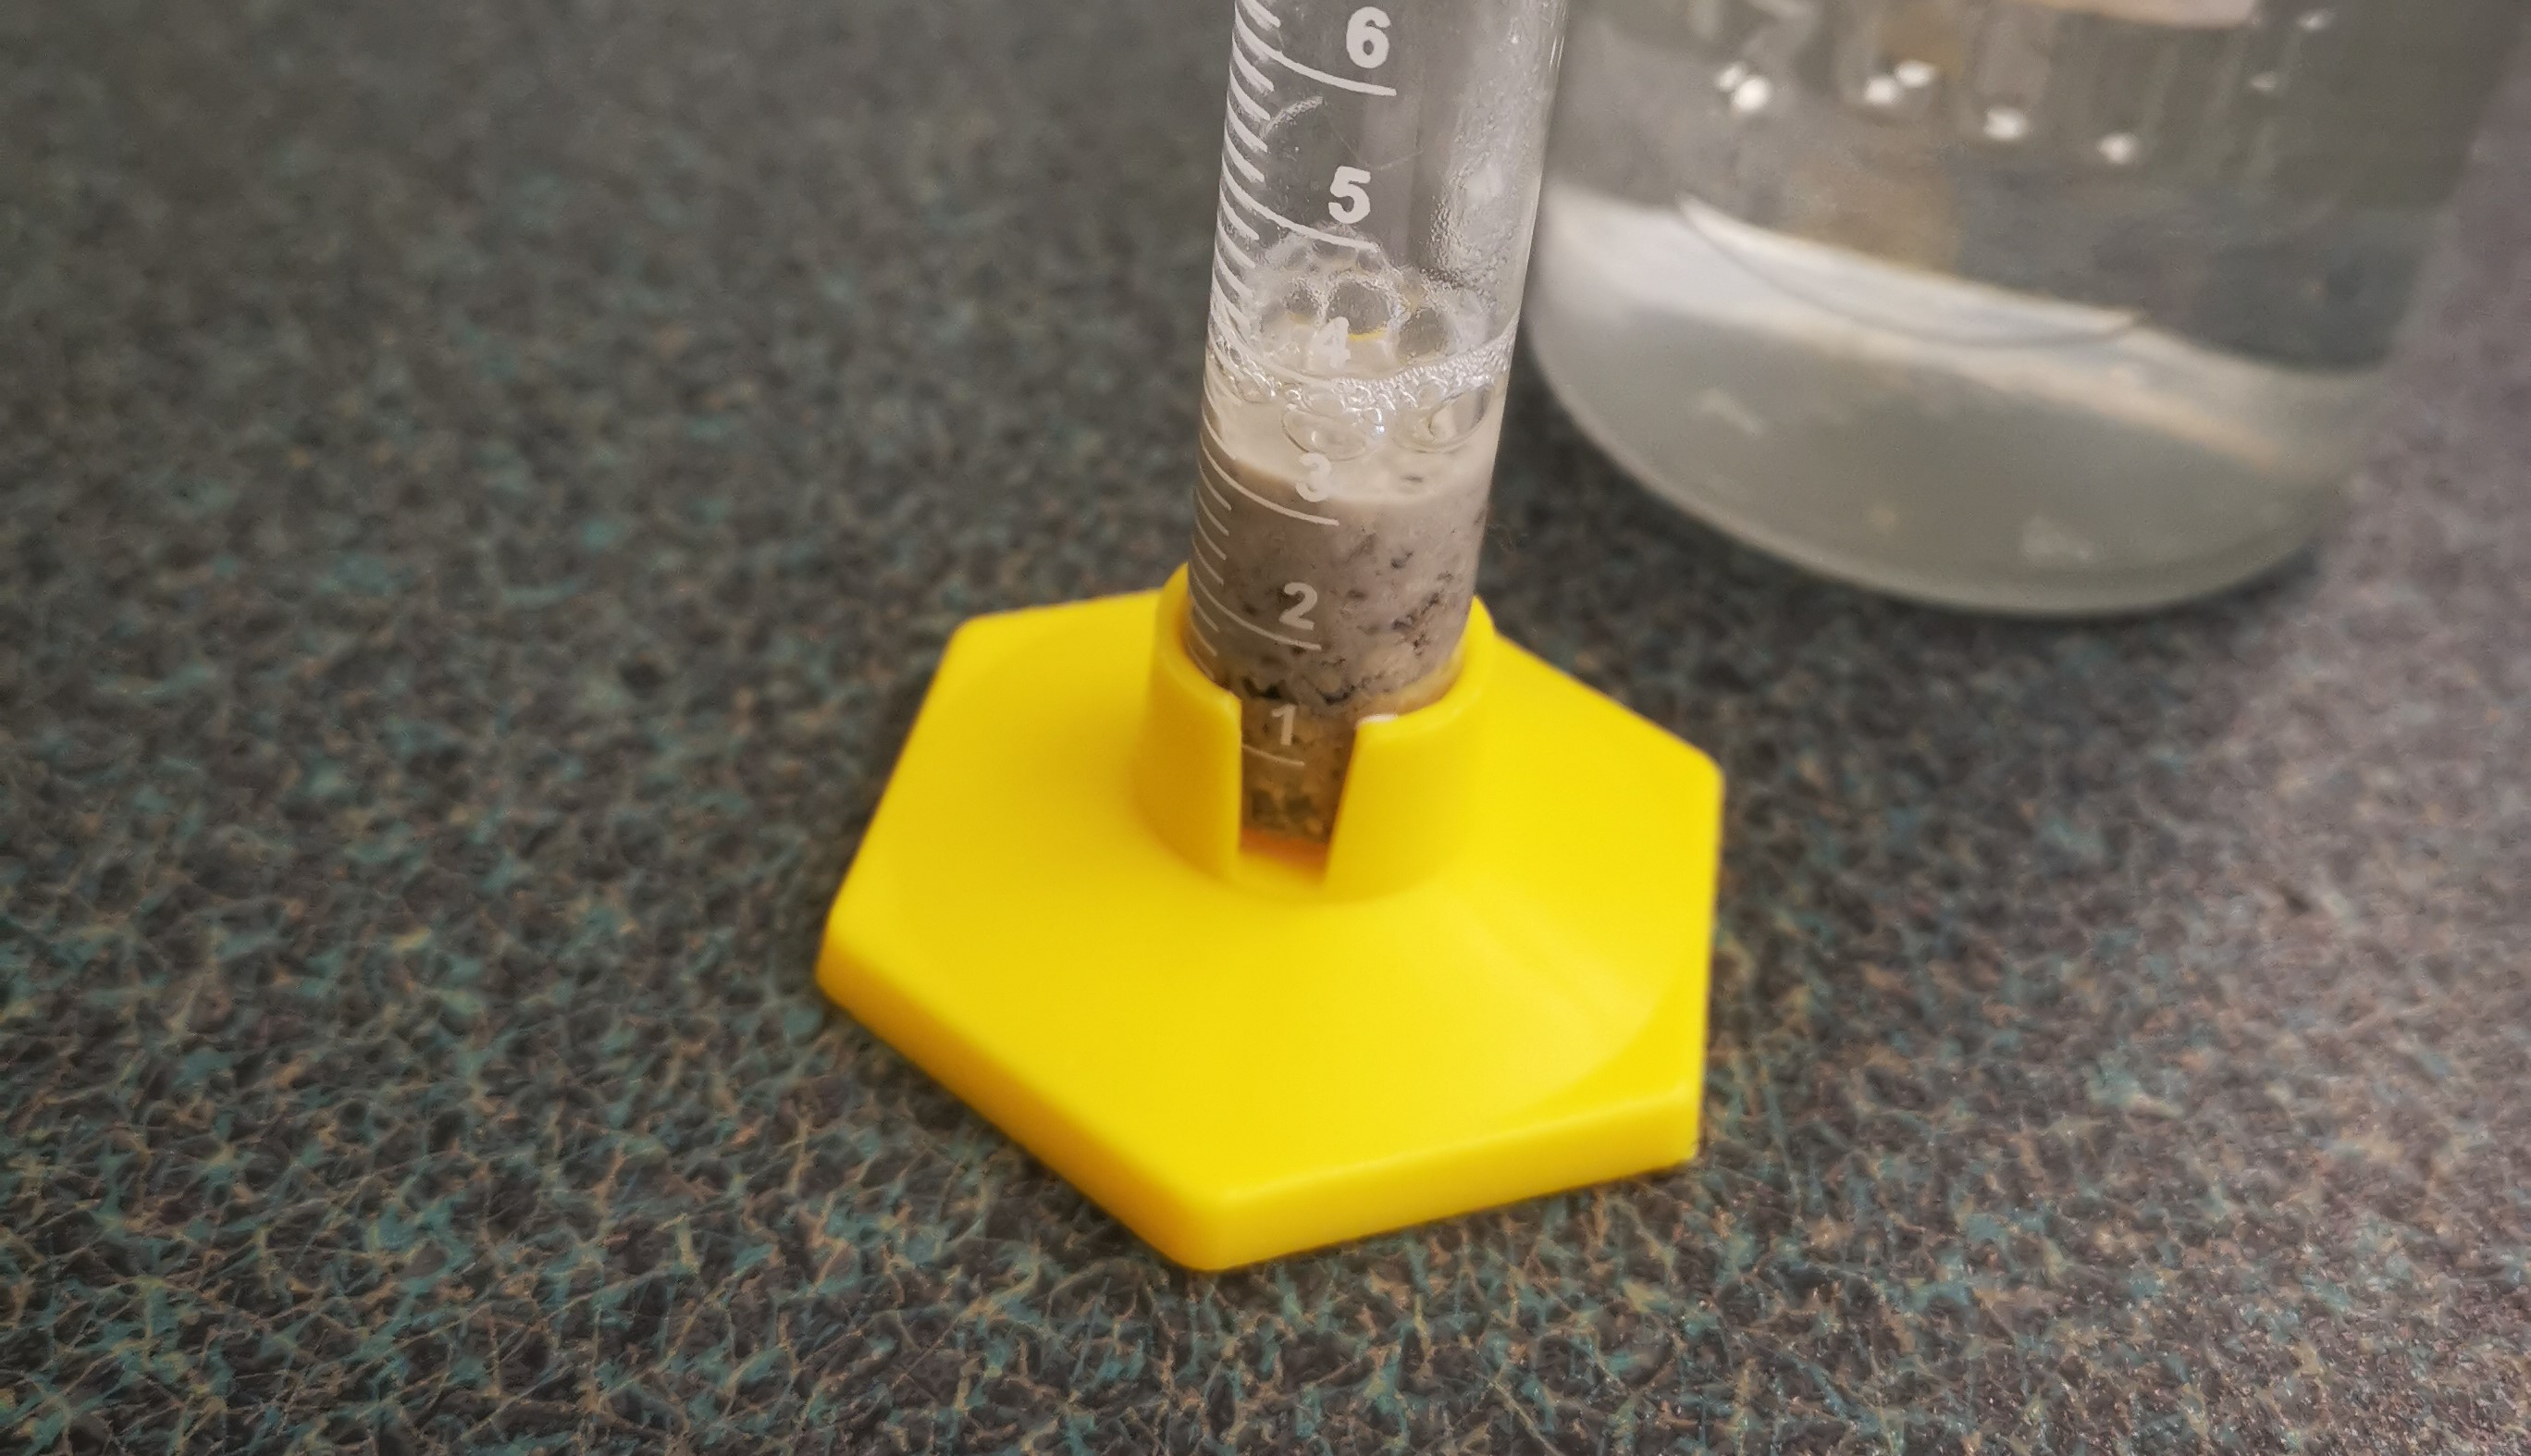
\includegraphics[width=0.28\textwidth]{poc1MHCL.jpg}
    \end{center}
    \caption{Proof of Concept Trial of \SI{1.0}{mL} \SI{1.0}{mol.dm^{-3}} \ce{HCl} with \SI{1.0}{mL} bentonite clay}
    \label{fig:poc1MHCL}
\end{wrapfigure}

Before the experiment was performed, a proof of concept
was done to determine whether there is a difference
in swelling between different concentrations and what the
range of concentrations should be in order to obtain
a holistic result.

Initially, two test trials were done where \SI{1.0}{mL} of
\SI{1.0}{mol.dm^{-3}} \ce{HCl} and \SI{1.0}{mL} of water
were each mixed into \SI{1.0}{mL} of bentonite clay in
\SI{10}{mL} graduated cylinders. In both mixtures, the
bentonite clay was not completely mixed with the solutions,
with virtually all the acidic solution being absorbed by the
clay as seen in Figure \ref*{fig:poc1MHCL}.

This heavy absorption of the clay was heavily problematic
for the actual experiment, as not only does it not ensure
complete absorption of the solution but also leads to difficulty
in cleaning out the mixture especially in a \SI{10}{mL} graduated
cylinder. On the packaging of the bentonite clay, it recommends
that the clay and solution should be mixed at a 1:10 ratio.

\begin{wrapfigure}{l}{0.28\textwidth}
    \begin{center}
        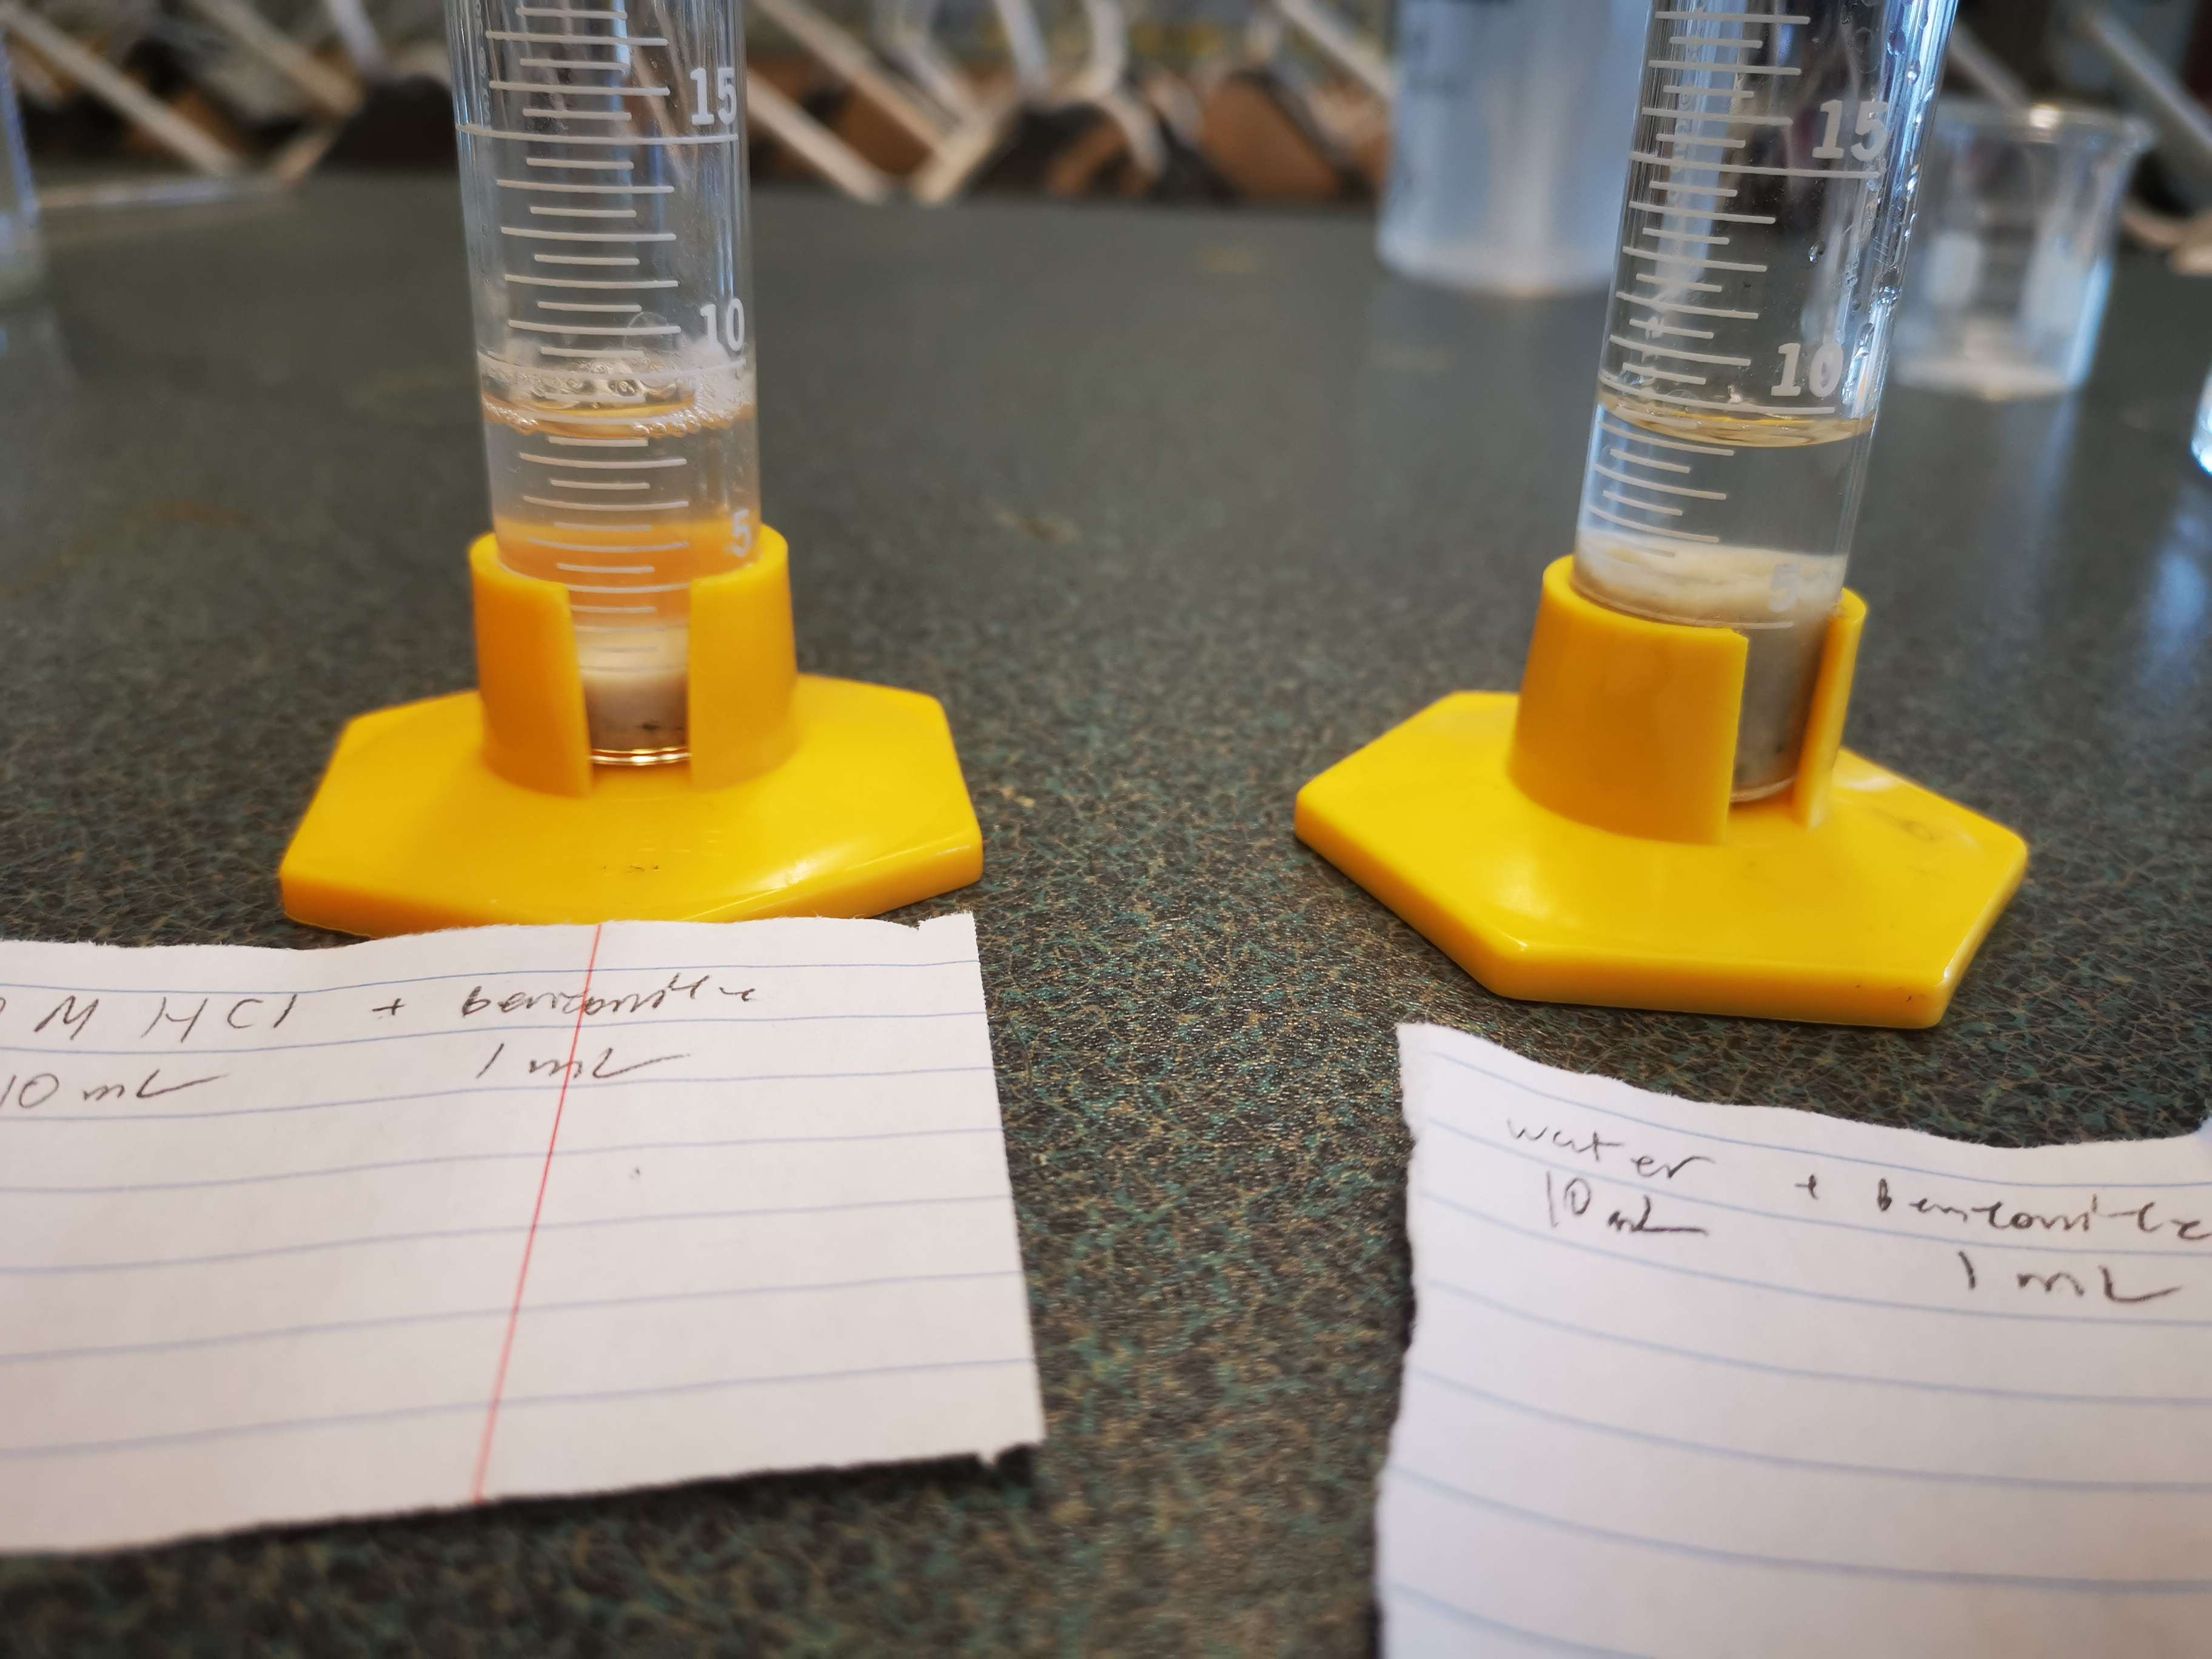
\includegraphics[width=0.28\textwidth]{betterPOC.jpg}
    \end{center}
    \caption{Proof of Concept Trial of \SI{10}{mL} \SI{1.0}{mol.dm^{-3}} \ce{HCl} (left) and \SI{10}{mL} of water (right) with \SI{1.0}{mL} bentonite clay}
    \label{fig:betterPOC}
\end{wrapfigure}

Two additional test trials were done with \SI{10}{mL} of
\SI{1.0}{mol.dm^{-3}} \ce{HCl} and \SI{10}{mL} of water,
each mixed into \SI{1.0}{mL} of bentonite clay in
\SI{25}{mL} graduated cylinders. Mixing between
bentonite clay and the solutions were way better with a
significant difference in swelling between the two mixtures
(the acid swelled the clay by a factor of about 3, while
the water swelled the clay by a factor of about 5.6).
These two test trials are shown in Figure \ref*{fig:betterPOC}.

It was at this point when there was the realization that it
is likely better to mix the clay into the solution rather than
the other way around to ensure optimal absorption of the solution
by the clay. However, what is to come next is determining the
best maximum \ce{[H+]} to see the optimal holistic result
in the relationship between the factor of swelling and \ce{[H+]}.
In this proof of concept, the method of mixing the solution
into the clay was continued to ensure that there is consistency
between the test trials.

\begin{wrapfigure}{R}{0.2\textwidth}
    \begin{center}
        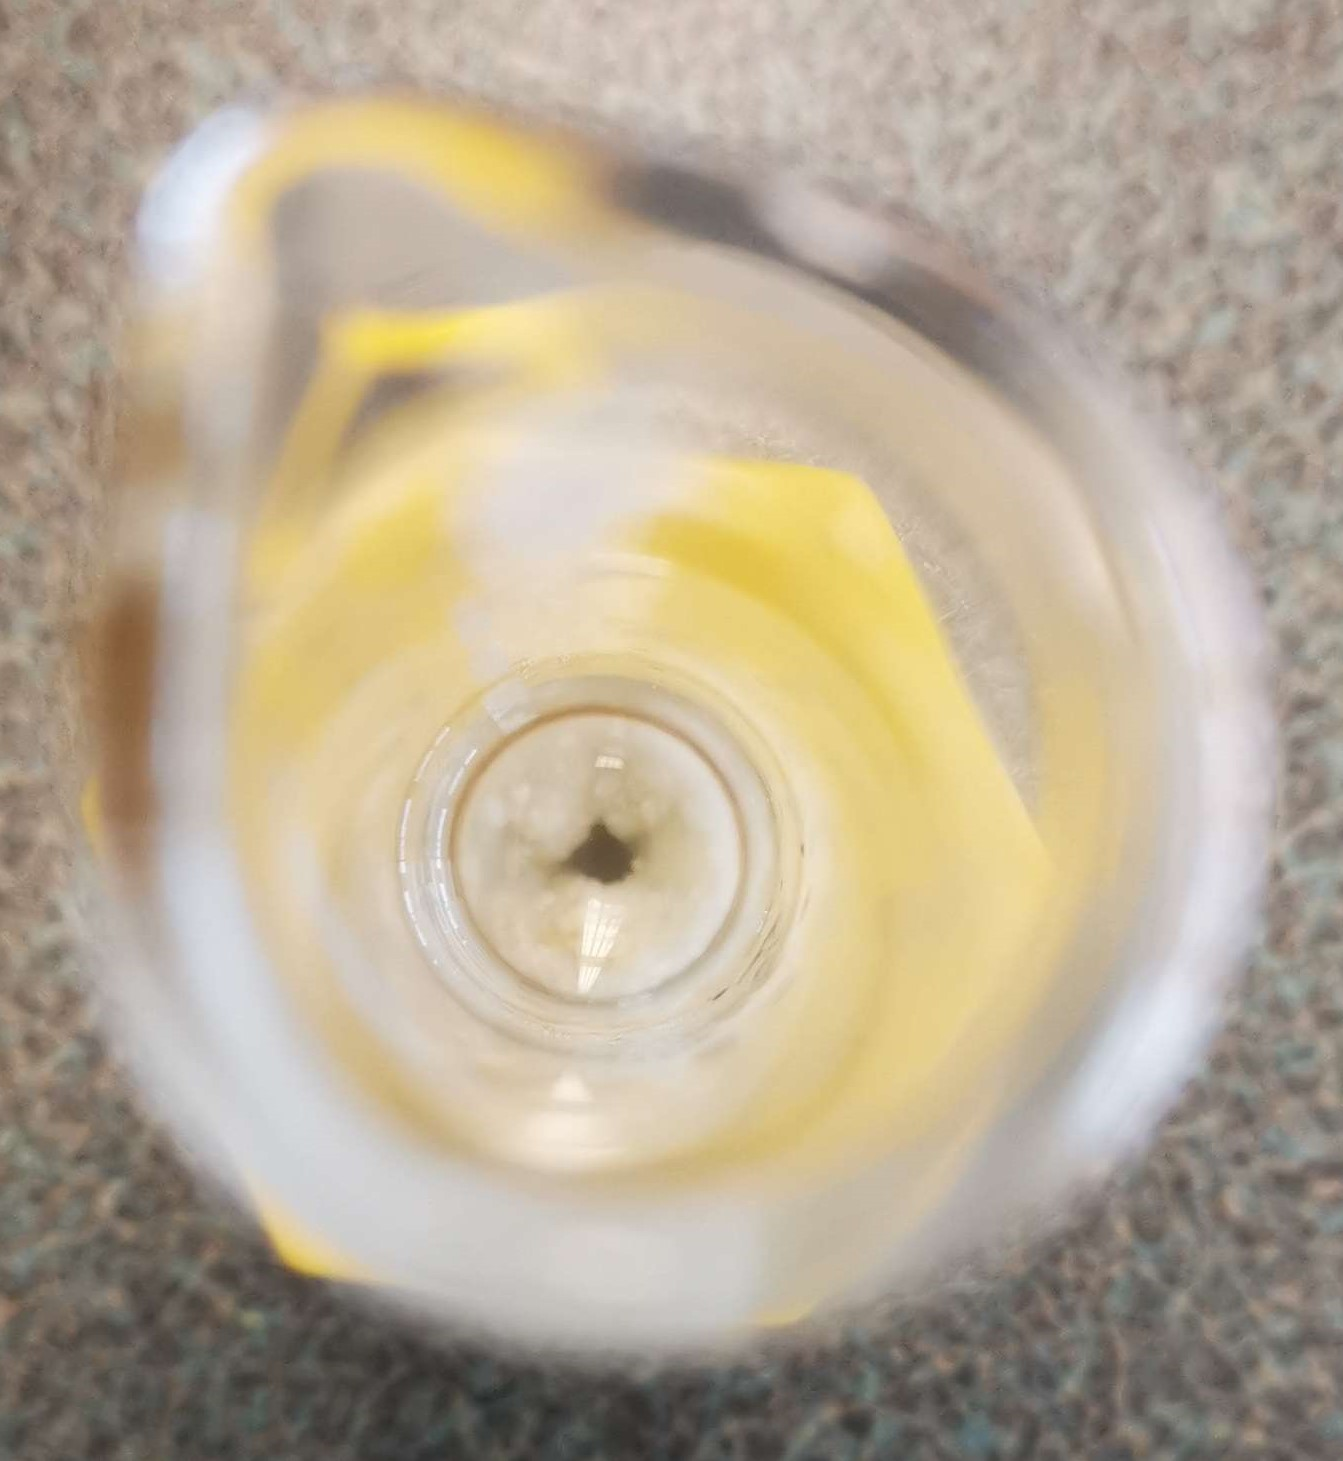
\includegraphics[width=0.18\textwidth]{hole.jpg}
    \end{center}
    \caption{Hole in bentonite clay in test trial between \SI{10}{mL} of water with \SI{1.0}{mL} bentonite}
    \label{fig:hole}
\end{wrapfigure}

One interesting qualitative observation at this point was that
in the mixture of bentonite clay with water, there was a hole
in the immersed bentonite clay, as seen in Figure \ref*{fig:hole}.

It is unknown why this occurs, but it may be suggested that
this could be as a result of mixing solution into the clay,
therefore mixing clay into the solution may mitigate this issue.

Finally, \SI{10}{mL} of \SI{2.0}{mol.dm^{-3}} was mixed with \SI{1.0}{mL}
of bentonite clay. The factor to which the bentonite had swollen by
in this mixture (2.8 times) doesn't differ much compared to the
mixture with \SI{10}{mL} of \SI{1.0}{mol.dm^{-3}} \ce{HCl}, therefore
it was decided that \SI{1.0}{mol.dm^{-3}} will be the maximum
concentration for this investigation.

\section{Hypothesis}

The hypothesis for this experiment is that the relationship between
the factor by which the volume of
sodium bentonite swells and the concentration of \ce{H+} ions of the mixed
solution will be indirectly proportional in linear fashion
given that a linear increase in \ce{[H+]} means a linear increase
of the amount of \ce{H+} ions that become available to replace \ce{Na+} ions.

However, it is predicted that there will be a point where
a decrease in swelling will begin to slow down when a deficiency
of \ce{Na+} ions in between the bentonite clay layers grows.
It is hypothesized that this effect will be manifested
as a horizontal asymptote on the plotted graph of the Factor
of swelling as a function of \ce{[H+]}.

\section{Variables}

\subsection{Manipulated Variable}
The manipulated variable is the pH of the solution mixed with the
bentonite clay. In this lab, the manipulated variable will be
changed by acid dilution.

\subsection{Responding Variable}
The responding variable is the factor by which the clay has swollen by.
The responding variable will be measured using a \SI{25}{mL} graduated cylinder.

\subsection{Controlled Variable 1: Clay swelling duration}
\subsubsection{How to control it}
For each trial, set a timer for a set amount of time and record
the final volume when the timer ends.
\subsubsection{Why it must be controlled}
Inconsistent durations of time between trials will entail
that the clays that were allows more time to swell will be able
to swell more than it should relative to the other trials.
Note that in the process, there will be a slight difference in duration
allowed between the 5 trials that share the same \ce{[H+]}.
This is not significant as due to the slow nature of clay swelling,
a difference in duration by under a minute will not lead to
major inconsistencies.

\subsection{Controlled Variable 2: Volume of initial clay}
\subsubsection{How to control it}
Consistently use a set volume of bentonite clay for each trial. Note
that because bentonite is rather sticky and therefore is tough
to clean out of a thin graduated cylinder, then it is best to
standardize the volume of clay committed for the experiment
by taking the volume of the dry bentonite with a graduated cylinder
and transferring it to a weigh boat to determine what mass of clay
is associative with the set volume of clay.
\subsubsection{Why it must be controlled}
Differing the volume of initial clay between trials will lead to
major differences in sodium ions present in the clay. This will
lead to inconsistencies of the swelling factor as there will
be more/less sodium ions ready to be exchanged with
hydrogen ions.

\subsection{Controlled Variable 3: Volume of solution mixed with clay}
\subsubsection{How to control it}
Measure the same volume of solution for each trial.
\subsubsection{Why it must be controlled}
Differing the volume of solution mixed with the clay between different
trials will lead to major difference of the amount \ce{H+} ions available to
be exchanged with \ce{Na+} ions in the clay. Because this ion
exchange is essential to the behaviour of swelling in bentonite clay,
the volume of the solution mixed with the clay must be controlled.

\section{Equipment and Materials}

\begin{multicols}{2}

    \begin{itemize}
        \item Lab Apron
        \item Lab Goggles
        \item Waste Beakers
        \item Distilled Water
        \item Sodium Bentonite Clay
        \item \SI{1.0}{mol.dm^{-3}} hydrochloric acid (HCl)
        \item \SI{0.1}{mol.dm^{-3}} hydrochloric acid (HCl)
        \item (1) \SI{10}{mL} Graduated Cylinder
        \item (5) \SI{25}{mL} Graduated Cylinders
        \item (3) \SI{100}{mL} Volumetric Flasks
        \item \SI{10}{mL} pipette
        \item (5) Weigh Boats
        \item Pipette pump
        \item Scoopula
        \item (2) Stir rod
        \item Paper towel
        \item Digital Balance
        \item Timer
    \end{itemize}

\end{multicols}

\section{Safety, Environmental, and Ethical Considerations}

\begin{itemize}
    \item Always remember to wear your lab apron and eye protection before proceeding with the experiment
    \item Read the Safety Data Sheet of hydrochloric acid before beginning the experiment
    \item Thoroughly wash any skin that has been in contact with hydrochloric acid
    \item When performing acid dilution, always add the acid into the water and not the other way around.
    \item Dispose of any waste containing acid to a waste beaker, labelling the beaker with contents and approximate \ce{[H+]}
    \item Take caution when attaching/detaching a pipette pump onto/from a pipette, ensuring that the distance between your two hands do not apply overwhelming torque onto the pipette
\end{itemize}

\section{Procedure}

\begin{enumerate}
    \item Put on lab apron and eye protection
    \item Using the \SI{10}{mL} pipette, transfer \SI{50}{mL} of distilled water to the \SI{100}{mL} volumetric flask \label{step:pip}
    \item Top up the \SI{100}{mL} volumetric flask with \SI{1.0}{mol.dm^{-3}} \ce{HCl} to obtain a \SI{100}{mL} solution of \SI{0.5}{mol.dm^{-3}} \ce{HCl} \label{step:mix}
    \item Repeat Steps \ref*{step:pip} and \ref*{step:mix} using \SI{0.1}{mol^{-3}} \ce{HCl} to obtain a \SI{100}{mL} solution of \SI{0.05}{mol.dm^{-3}} \ce{HCl}
    \item Using the \SI{10}{mL} pipette, transfer \SI{10}{mL} of distilled water to the \SI{100}{mL} volumetric flask
    \item Top up the \SI{100}{mL} volumetric flask with \SI{1.0}{mol.dm^{-3}} \ce{HCl} to obtain a \SI{100}{mL} solution of \SI{0.01}{mol.dm^{-3}} \ce{HCl}
    \item Using a scoopula, transfer bentonite clay into the \SI{10}{mL} graduated cylinder until there is \SI{1}{mL} of bentonite clay
    \item Place a weigh boat onto the digital balance and tare the balance
    \item Transfer all the bentonite clay in the \SI{10}{mL} graduated cylinder into the weight boat and record the mass of the bentonite clay \label{step:findClayMass}
    \item \label{step:measureMass} Place another weight boat on the digital balance, tare the balance, then transfer enough bentonite clay using the scoopula such that the mass read by the balance matches the mass found in Step \ref*{step:findClayMass}.
    \item Repeat Step \ref*{step:measureMass} for all 5 weigh boats.
    \item Using the \SI{10}{mL} pipette, transfer \SI{10}{mL} of a solution to each \SI{25}{mL} graduated cylinder
    \item Flick the bottom of each weight boat such that all the clay reaches to one corner, then proceed to transfer the clay of each weigh boat to each \SI{25}{mL} graduated cylinder as quickly as possible
    \item Set a timer for 10 minutes
    \item As the timer approaches its end, start flicking each graduated cylinder to force all the bentonite clay to be submerged at the bottom of the graduated cylinder
    \item Once the timer ends, record the final volumes of bentonite clay in each \SI{25}{mL} graduated cylinder
    \item If the solution is acidic, first transfer remaining solution into the waste beaker, using an acid designated stir rod to remove the majority of the clay. Fill up the graduated cylinder with water, then transfer the water and any large chunks of clay into the waste beaker again
    \item \label{step:clean} Repeatedly fill the graduated cylinder with water and scrub the interior with a stir rod wrapped by paper towel until no clay remains
    \item Repeat Steps \ref*{step:measureMass} to \ref*{step:clean} for all solutions
    \item Wash your hands thoroughly after the experiment and clean the laboratory workspace
\end{enumerate}

\section{Evidence}
\subsection{Qualitative Observations}
\subsection{Quantitative Data}

\section{Processed Data}

\section{Analysis}

\section{Evaluation}

% \end{multicols*}

\bibliographystyle{apacite}
\bibliography{IB_CHEM_IA.bib}

\end{document}